\subsection{Предварительная обработка изображения} \label{part2.2.1}
\subsubsection{Фильтрация изображений с помощью гауссового фильтра}
Шум является неотъемлемой частью любого устройства регистрации изображений и видео. Условно можно выделить следующие виды шума:

\begin{itemize}
	\item Шум  устройств захвата изображения;
	\item Смаз изображения, связанный с условиями регистрации, включая скорость и траекторию движения камеры;
	\item Независимый случайный шум;
	\item Отдельно отметим вмешательство наблюдения объектов.
\end{itemize}

В основе математической теории обработки изображений, включая фильтрацию, лежит понятие свертки (convolution) c определенным ядром (kernel, маска фильтра). Для того, чтобы выполнить преобразование была проведена «свертка» входного изображения с соответствующим (заранее выбранным) ядром. Со всеми пикселями в изображении проводятся свертка с ядром свертки (\ref{eq1}) (центр окна свертки будет размещен в позиции пикселя, вычисляется свертка), изменение исходных значений пикселей.
\begin{equation}\label{eq1}
Y\left(m,n\right)=X\left(m,n\right)\ast H\left(k,l\right)=\sum^r_{k=-r}\sum^r_{l=-r}X\left(m-k,n-l\right)H\left(k,l\right),
\end{equation}

\begin{itemize}
	\item $X\left(m,n\right)$ - исходная матрица размера изображения $m\ast n$;
	\item $H\left(k,l\right)$ - матрица ядра свертки, также известная как маска;
	\item $Y\left(m,n\right)$ - выходная матрица свертки между $X$ и $H$.
\end{itemize}

В данной работе использован фильтр Гаусса для удаления шума. Сущность этого преобразования состоит в реализации свертки оригинального изображения с ядром симметричной формы в виде 2-D функции Гаусса. Эта непрерывная функция определяется следующим образом:
\begin{equation}\label{eq2}
f\left(x,y\right)=\frac{1}{2\pi\sigma^2}exp\left(-\frac{x^2+y^2}{2\sigma^2}\right).
\end{equation}

Теория линейной и нелинейной фильтрации изображений является областью проведения активных научных исследований \cite{Sizikov2011,Sizikov260,Sizikov2012}.
\subsubsection{Метод бинарной морфологии}
В настоящее время методы цифровой обработки изображений привлекли внимание многих исследователей и разработчиков. Отдельно отметим метод морфологической обработки изображений.

Морфологическая обработка изображений дает количественное описание структуры и геометрии объектов в изображении, основанной на математической теории, таких как теории множеств, топологии, теории вероятности и т.д.

В приложениях компьютерного зрения морфологическая обработка используется для идентификации объектов, повышении качества изображения, сегментации изображения и проверки ошибок на изображении. Операции морфологической обработки выполняются в основном на бинарном изображении.

\textbf{Структурные элементы} \cite{Burger2009}.  В бинарном изображении, Структурный элемент представляет собой небольшое изображение, состоящий из двух значений $0$ и $1$, при этом $0$ значения игнорируются в процессе вычисления, $H\left(i,j\right)$ является структурные элементы бинарного изображения и выражается следующим образом: $H\left(i,j\right) \in \left\{0,1\right\}$.

Некоторые формы структурных элементов, обычно используемые в бинарном изображении: горизонтальные и вертикальные линии, квадраты, эллипсы и пр.

\begin{figure}[ht!]
\centering
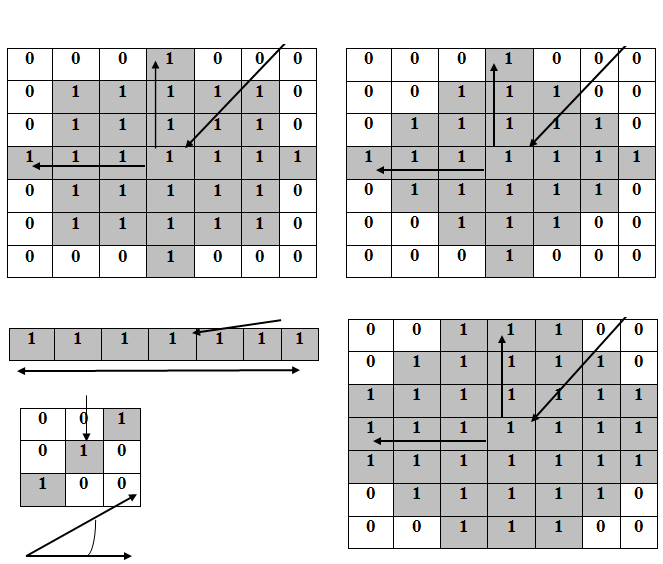
\includegraphics [scale=0.8] {images/h8.png}
\begin{center}
%\captionsetup{justification=justified, labelsep=period}
\caption{Описание формы структурных элементов.} \label{img8}
\end{center}
\end{figure}
Цель метода морфологической обработки - найти связанные компоненты контура объекта для получения идеального контура.

Операции дилатации, эрозии, открытия и закрытия могут быть применены для серого изображения. Эта концепция аналогична для бинарных морфологических операций.
\begin{equation}\label{eq3}
 g=\left(f\oplus b \right)-\left(f\ominus b\right),
\end{equation}
Где:

\begin{itemize}
	\item $f\oplus b$ является преобразованием расширения растяжением $f$ по структурным элементам b в положении $\left(x,y\right)$ по формуле:
	\begin{equation}\label{eq4}
\left[f\oplus b\right]\left(x,y\right)=max_{\left(s,t\right)\in b}\left\{f\left(x-t,y-t\right)\right\}.
\end{equation}
\item $f \ominus b$ является преобразованием эрозии растяжением $f$ по структурным элементам b в положении $\left(x,y\right)$ по формуле:
	\begin{equation}\label{eq5}
\left[f \ominus b\right]\left(x,y\right)=max_{\left(s,t\right)\in b}\left\{f\left(x+t,y+t\right)\right\}.
\end{equation}
\end{itemize}
Набор пикселей, которые соединяются с другими называется компонентой связности \cite{Solomon2011}. Пиксели соединены друг с другом, которые отличаются от других групп пикселей назначенной им меткой. Эти метки представляют собой целые числа, где фон имеет значение $0$, область изображения $/$ группа взаимосвязанных пикселя помечена $1$.
\begin{figure}[ht!]
\centering
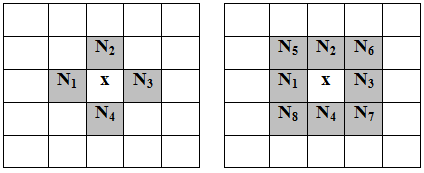
\includegraphics [scale=0.8] {images/h9.png}
\begin{center}
%\captionsetup{justification=justified, labelsep=period}
\caption{Форма 4 соседей (N4) и 8 соседей (N8).} \label{img9}
\end{center}
\end{figure}
В данной работе используются алгоритмы для обозначения 8-связных компонент (рис.\ref{img9}). Алгоритм включает в себя следующие этапы:

\begin{itemize}
	\item Шаг 1: Сканирование входных изображений последовательно по строкам сверху-внизу, чтобы встретить любую точку $p$ $\left(p=1,если бинарное изображен\right)$ в изображении;
	\item Шаг 2: Проверка соседей $p$. На основе этой информации, метка будет осуществляться следующим образом:
	
	\begin{itemize}
		\item Если все соседи со значением равным нулю, то $p$ присваивается новая, ранее не использовавшаяся метка.
		\item Если имеется только один соседний пиксел $р$ со значением $1$, присваиваем эту метку пикселу $р$;
		\item Если имеется больше чем один соседний пиксел $р$ со значением $1$, присваиваем метку любого из уже пронумерованных пикселов.
	\end{itemize}
	
\end{itemize}
После завершения процесса сканирования, соответствующие пары метки располагаются в соответствующие группы, и каждой группе будет присвоена только одна метка.
\subsubsection{Метод выравнивания гистограммы}
При регистрации изображений и видео при помощи всегда происходит дисбаланса света. Эта проблема может быть легко решена путем воздействия на источник света в случае лабораторных условиях регистрации.

Настоящая работа направлена на создание практических приложений для смартфонов, которые могут работать в реальных условиях освещения. Таким образом, автоматический баланс яркости является необходимым требованием для разрабатываемого комплекса программ. Используется метод эквализации гистограммы для решения задачи.

Эквализация гистограммы является простой теорией и часто используется при обработке изображений. Цель эквализации гистограммы, как уже отмечалось выше, заключается в увеличении диапазона яркости изображения.

Эквализация гистограммы изображения g определяется следующим образом:
\begin{equation}\label{eq6}
g_{i,j}=floor\left(\left(L-1\right)\sum^{f_{i,j}}_{n=0}p_n\right),
\end{equation}
Где:

\begin{itemize}
	\item $f$ - исходное изображение;
	\item $n=0,1,…,L-1;L \in \left[0 ; 255\right]$;
	\item $p_n$:Количество пикселей по интенсивности  n / Количество пикселей;
	\item $floor()$ округляется до ближайшего целого числа. Это эквивалентно преобразованию интенсивности пикселей, $k$, $f$ с помощью функции:
	\begin{equation}\label{eq7}
T\left(K\right)=floor\left(\left(L-1\right)\sum^k_{n=0}p_n\right).
\end{equation}
\end{itemize}
Этот метод имеет преимущество простоты, легкости применения, без каких-либо серьезных расчетов, он используется в случаях, когда необходимо привести изображение в его <<нормальное>> состояние.
